\documentclass[../xlapes02]{subfiles}



\begin{document}
    \chapter{Experiments and Results}\label{ch:experiments-and-results}
    In this section we present the results of all the experiments performed. We will also discuss any problems that arose during the conduct of these experiments and provide further information on how we selected certain methods and hyperparameters for more extensive testing.

    By performing a series of experiments, we show how our agent performs in a given environment. We compare the best and worst performing models and discuss the results of our experiments with the baseline models and benchmarks in~\cref{sec:experiments}. We also discuss and compare the hyperparameter settings and the advantages and disadvantages of all the datasets used in~\cref{subsec:hyperparameters}. We also provide some information on how we approached performance testing of the proposed models and what technologies were used for the MLOps concepts, such as tracking training and test runs~\cref{sec:wandb}. Finally, we discuss the results of our experiments and provide a summary of our findings~\cref{sec:summary}.
    \\
    \\
    The computer used for experiments has the following specifications:
    \begin{itemize}
        \item Operating System: Ubuntu 20.04.6 LTS (GNU/Linux 5.4.0-146-generic x86\_64)
        \item CPU: 2 x Intel Xeon CPU E5-2620 v3 @ 2.40GHz, each with six cores, for a total of 12 cores.
        \item RAM: 2 x 32 GB RAM running at 2133MHz, using quad-channel architecture for faster memory access
        \item GPU: 4 x NVIDIA GTX 1080 (Pascal) with 8GB RAM each, providing a total of 32GB GPU memory.
    \end{itemize}


    \section{Focus of the experiments}\label{sec:focus-of-the-experiments}
    In~\cref{ch:stock-portfolio-allocation}, we implement the \emph{Stock Portfolio Allocation Environment}, while in the this chapter, we conduct experiments to \emph{evaluate} the trained models. Our aim is to determine the best \emph{parameters} and \emph{datasets} for training and testing. To achieve this, we use a \emph{sweeping} approach to test the hyperparameters for each algorithm and dataset. We evaluate each configuration of hyperparameters in terms of the model's performance, which is measured by the total reward calculated as the cumulative product of the portfolio value.

    We compare the best and worst performing models with other models and common indexes as baselines. Our results indicate that appropriate hyperparameters and datasets can train the agent sufficiently well to outperform common indexes and other publicly available models for Portfolio Allocation (using Reinforcement Learning). This makes them valuable tools for portfolio allocation in financial markets.

    Thus, the main goal of this chapter is to evaluate the trained models' performance through rigorous experimentation and identify the best \emph{parameters} and \emph{datasets} for optimal performance. We also test the model's \emph{robustness} by assessing its stability using the best hyperparameters for the datasets and the specific algorithm used to train the model. This helps us ensure that the model is reliable and can perform consistently well under different conditions. The robustness test helps us identify potential weaknesses or limitations that may need to be addressed.

    \subsection{Reproducing Results}
    Furthermore, not only do we provide the results of our work in this thesis, but we also make all datasets and training runs with a history of hyperparameters for each algorithm publicly available on the W\&B website. \textbf{By visiting the following URL: \url{https://wandb.ai/investai/portfolio-allocation}}, anyone can access the results of each run, including the stored models and datasets, and reproduce our findings while comparing them with their own experiments.


    \section{Weights \& Biases}\label{sec:wandb}
    Weights \& Biases (W\&B) is a powerful machine learning experiment tracking and visualization tool that helps data scientists and machine learning practitioners manage their experiments. With W\&B, users can log experiment metrics in real-time, track hyperparameters, and compare and reproduce experiments easily. W\&B offers various visualization tools like interactive plots, histograms, and confusion matrices, which help users analyze and understand experiment results.

    \begin{itemize}
        \item Experiment tracking: W\&B allows users to log experiment metrics such as loss, accuracy, and other custom metrics in real-time during training. These metrics are logged to a central dashboard, making it easy to monitor and compare multiple experiments.
        \item Hyperparameter tuning: W\&B supports hyperparameter sweeps, allowing users to explore different hyperparameter configurations in parallel and find optimal hyperparameter settings for their models.
        \item Visualization: W\&B provides a variety of visualization tools, including interactive graphs, histograms, confusion matrices, and more, to help users analyze and understand experimental results. We use some of the W\&B graphs to compare hyperparameters and their values to understand their effect on the overall range of rewards~\crefrange{fig:wb-chart1}{fig:wb-chart3}.
        \item Artifact management: W\&B allows users to log and version datasets, models, and other artifacts, making it easy to track and reproduce experiments with specific data and model versions.
        \item Collaboration: W\&B enables team collaboration by allowing users to share experiment results, visualizations, and artifacts with team members, facilitating communication and collaboration among team members.
    \end{itemize}

    Since the W\&B API offers a number of features, we decided to focus on experiments and not describe them all. However, we recommend to consult the W\&B documentation available at \url{https://docs.wandb.ai/} for an explanation of all APIs and features, and to see the results of our experiments with all artifacts at \url{https://wandb.ai/investai/portfolio-allocation}.


    \section{Experiments}\label{sec:experiments}
    All experiments are focused on several metrics. The first is whether the model can outperform standard indices such as the S\&P 500 Index, DJI Index and others. Second, what dataset is more appropriate for training the model. Finally, assessing the robustness of the model. All experiments will be documented during our testing period, which spans from \emph{2017-01-25} to \emph{2022-12-16}. As the datasets are derived from \emph{companies in the DJI Index}, we will primarily compare the performance of our models with the DJI Index to maintain consistency in the results. However, we will also make comparisons with other indices.

    \subsection{Baselines and Backtesting}\label{subsec:baselines-and-backtesting}
    In this subsection, we compare the performance of the agent to several baselines, including well-known market indexes and investment strategies. The following strategies and indexes were used as baselines:

    \begin{itemize}
        \item \textbf{The S\&P 500 Index (GSPC)} is a capitalization-weighted index that tracks the performance of 500 large publicly traded companies in the US. The index is maintained by S\&P Dow Jones Indices and is one of the most widely followed equity indices.
        \item \textbf{The Dow Jones Industrial Average (DJI)} is a price-weighted index that tracks the stock performance of 30 large companies listed on US stock exchanges. It is also one of the most commonly followed equity indices.
        \item \textbf{The Russell 2000 (RUT)} is a stock market index that tracks the performance of 2,000 small-cap companies in the US. It is a subset of the Russell 3000 index, which represents about 98\% of the total market capitalization of the US equity market.
        \item \textbf{The NASDAQ Composite (IXIC)} is a stock market index that tracks the performance of all the companies listed on the NASDAQ stock exchange, which is primarily composed of technology and growth-oriented companies. It is one of the most widely-followed stock market indices in the world.
        \item \textbf{Minimum Variance} is a portfolio allocation strategy that aims to minimize the variance of the portfolio's returns. The strategy assumes that the variance of the portfolio's returns is a measure of risk~\cite{investopedia}.
        \item \textbf{Maximum Sharpe Ratio} is a portfolio allocation strategy that aims to maximize the Sharpe ratio of the portfolio. The strategy assumes that the Sharpe ratio is a measure of risk-adjusted return~\cite{investopedia}.
    \end{itemize}

    \subsubsection{Cumulative Returns}
    In \cref{fig:cumulative_return}, we demonstrate that an agent can achieve successful outcomes when trained with appropriate hyperparameters and dataset (model id: \emph{zfjr0ks0}), while unsuitable hyperparameters and dataset can result in unsatisfactory outcomes (model id: \emph{p3irnh80}). The \emph{zfjr0ks0} model surpassed standard indexes such as DJI, GSPC, IXIC, and RUT, although not consistently throughout the testing period. It is evident that the \emph{zfjr0ks0} model outperformed almost all baseline indexes and strategies, with the exception of \emph{IXIC} (Nasdaq 100 Index) during a specific period from 2020 until the end of the testing period in 2022, when our model began to outperform even \emph{IXIC}. This is a simple comparison between the model with the best and worst performance. Later, we will also compare our model with the one from \emph{AI4Finance}, but we currently lack the data to perform a full comparison over our entire testing period.
    \begin{figure}[h!]
        \centering
        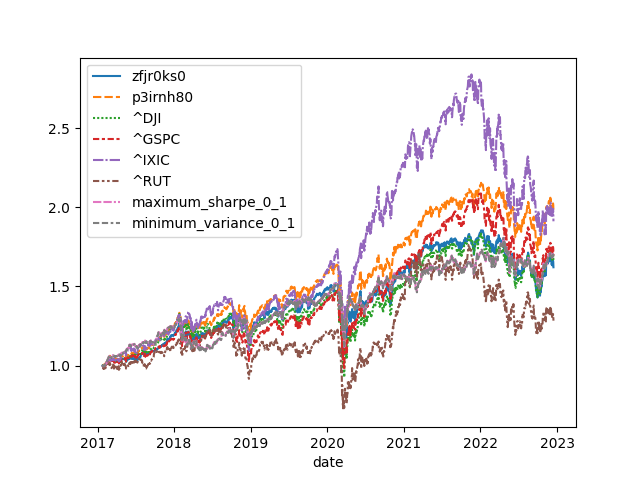
\includegraphics[width=\linewidth]{image/figure/returns}
        \caption{Cumulative returns of the best(zfjr0ks0) and worst(p3irnh80) performing models, indexes (DJI, GSPC, IXIC, RUT), and strategies (minimum variance and maximum Sharpe ratio), during the testing period (2017-2022).}
        \label{fig:cumulative_return}
    \end{figure}

    \subsubsection{Drawdowns}
    Now we look how our models performing in drawdowns\footnote{In the stock market, drawdown refers to the percentage decline in an investment's value from its peak to its subsequent low point. Essentially, it represents the loss experienced by an investor in a particular investment over a certain period of time.} Based on the drawdown graphs in~\cref{fig:drawdown}, we observe that the best model, trained on appropriate datasets and hyperparameters, outperforms the DJI index for larger drawdowns (around $6\%$). Since our dataset comprises companies included in the DJI index we decide for our analysis compare the drawdowns of the model with the \emph{highest and lowest test/total\_reward}, as well as \emph{two indexes} (\emph{IXIC} and \emph{DJI}). The \emph{IXIC} (Nasdaq 100 Index) has been chosen as baseline for performance in drawdown, since it outperformed our model during the period between 2020 and 2022.

    \begin{figure}[h!]
        \begin{subfigure}[t]{\experimentimgwidth\textwidth}
            \centering
            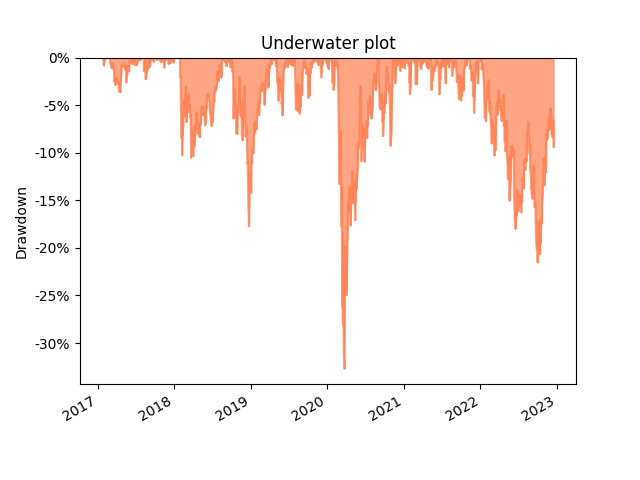
\includegraphics[width=\linewidth]{image/figure/drawdown_underwater_max}
            \caption{The model with the highest \emph{text/total\_reward}}
            \label{fig:drawdown_underwater_max}
        \end{subfigure}
        \hfill
        \begin{subfigure}[t]{\experimentimgwidth\textwidth}
            \centering
            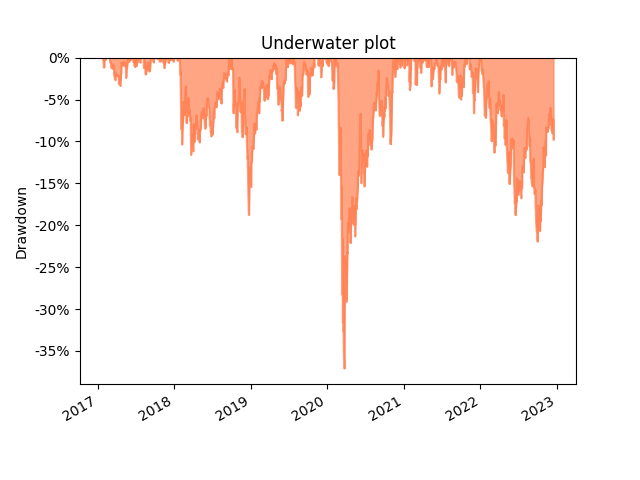
\includegraphics[width=\linewidth]{image/figure/drawdown_underwater_dji}
            \caption{The DJI index}
            \label{fig:drawdown_underwater_dji}
        \end{subfigure}

        \vspace{0.5cm}

        \begin{subfigure}[t]{\experimentimgwidth\textwidth}
            \centering
            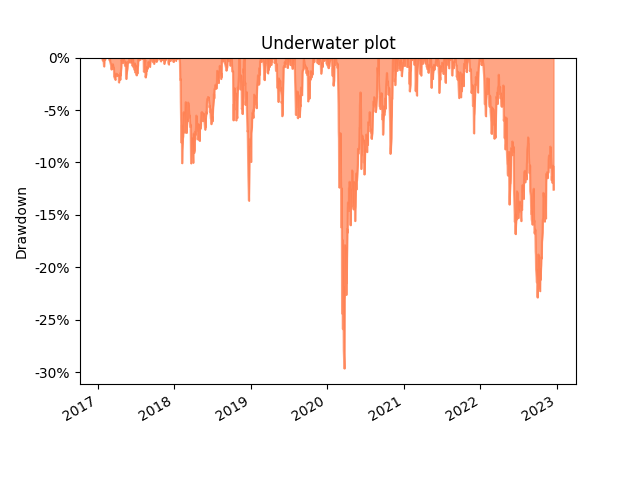
\includegraphics[width=\linewidth]{image/figure/drawdown_underwater_min}
            \caption{The model with the lowest \emph{text/total\_reward}}
            \label{fig:drawdown_underwater_min}
        \end{subfigure}
        \hfill
        \begin{subfigure}[t]{\experimentimgwidth\textwidth}
            \centering
            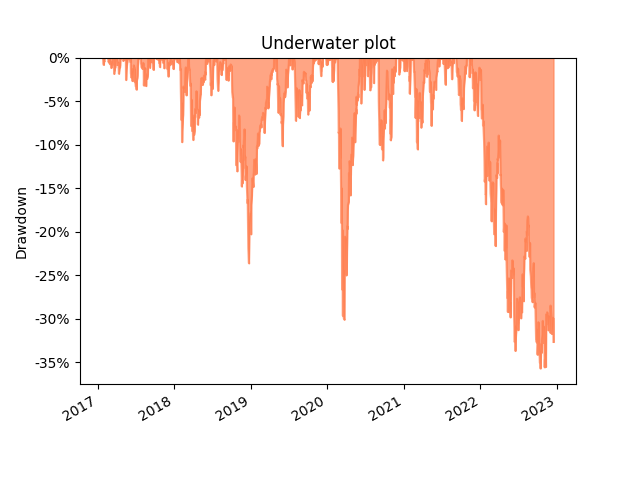
\includegraphics[width=\linewidth]{image/figure/drawdown_underwater_ixic}
            \caption{The IXIC index (Nasdaq 100 Index)}
            \label{fig:drawdown_underwater_ixic}
        \end{subfigure}

        \caption{Drawdown.}
        \label{fig:drawdown}
    \end{figure}

    \subsubsection{Monthly and Annual Returns}
    In figure \cref{fig:month_annual_returns}, both the monthly and annual returns of the models are presented, allowing for easy comparison of their performance. The results are similar to the cumulative returns described in the previous subsubsection, but the monthly returns provide a clearer understanding of when the models performed well or poorly. The model with the highest \emph{text/total\_reward} consistently outperforms the DJI index in most months, while even the model with the lowest \emph{text/total\_reward} performs better than the DJI index in the majority of months.

    Notably, the models achieved significant outperformance during the big drawdown period, as shown in the heatmaps in subfigures \cref{subfig:montly_returns_heatmap_max} and \cref{subfig:montly_returns_heatmap_dji}. Specifically, the model with the highest \emph{text/total\_reward} performed better than the DJI index during the COVID-19 pandemic months of February, March and April 2020, due to the differing company weightings in the DJI index. This suggests that our model was able to learn which companies with specific features were better to hold during this period.

    While there were some months where the DJI index performed better than our models, such as in April and October 2022, the performance difference was not significant. Therefore, we can conclude that our models performed well in the majority of months, as demonstrated by the annual graphs in subfigures \cref{subfig:annual_returns_max} and \cref{subfig:annual_returns_dji}.

    \begin{figure}[h!]
        \centering
        %
        \begin{subfigure}[t]{\experimentimgwidth\textwidth}
            \centering
            \label{subfig:montly_returns_heatmap_max}
            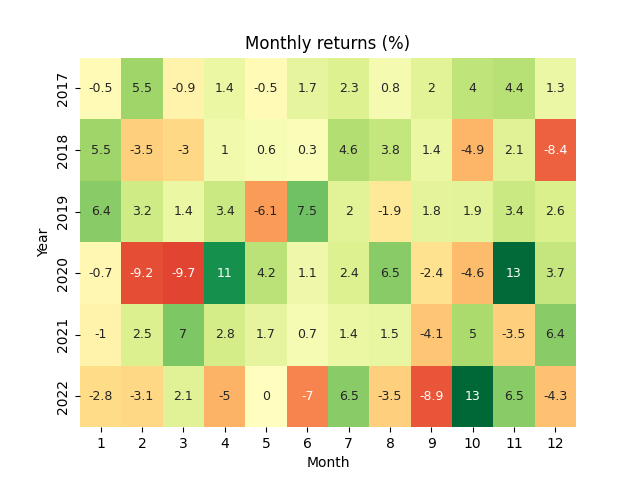
\includegraphics[width=\linewidth]{image/figure/monthly_returns_heatmap_max}
            \caption{The model with the highest \emph{text/total\_reward}}
        \end{subfigure}
        \hfill
        \begin{subfigure}[t]{\experimentimgwidth\textwidth}
            \centering
            \label{subfig:annual_returns_max}
            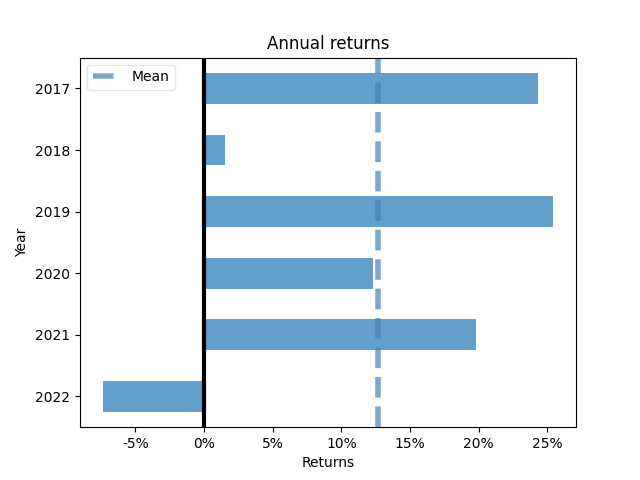
\includegraphics[width=\linewidth]{image/figure/annual_returns_max}
            \caption{The model with the highest \emph{text/total\_reward}}
        \end{subfigure}

        %
        \begin{subfigure}[t]{\experimentimgwidth\textwidth}
            \centering
            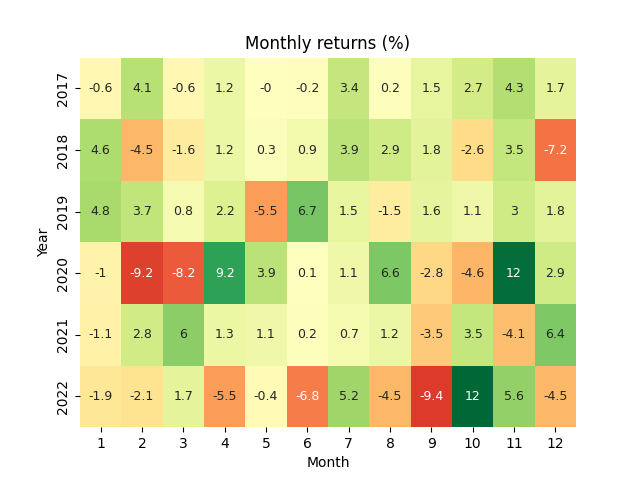
\includegraphics[width=\linewidth]{image/figure/monthly_returns_heatmap_min}
            \caption{The model with the smallest \emph{text/total\_reward}}
        \end{subfigure}
        \hfill
        \begin{subfigure}[t]{\experimentimgwidth\textwidth}
            \centering
            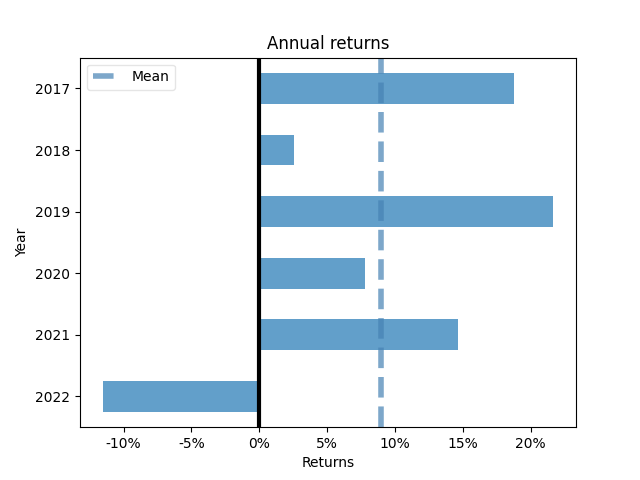
\includegraphics[width=\linewidth]{image/figure/annual_returns_min}
            \caption{The model with the smallest \emph{text/total\_reward}}
        \end{subfigure}

        %
        \begin{subfigure}[t]{\experimentimgwidth\textwidth}
            \centering
            \label{subfig:montly_returns_heatmap_dji}
            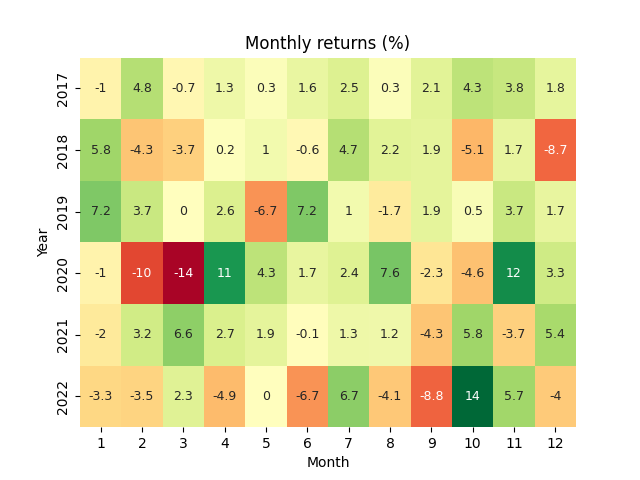
\includegraphics[width=\linewidth]{image/figure/monthly_returns_heatmap_dji}
            \caption{The DJI index}
        \end{subfigure}
        \hfill
        \begin{subfigure}[t]{\experimentimgwidth\textwidth}
            \centering
            \label{subfig:annual_returns_dji}
            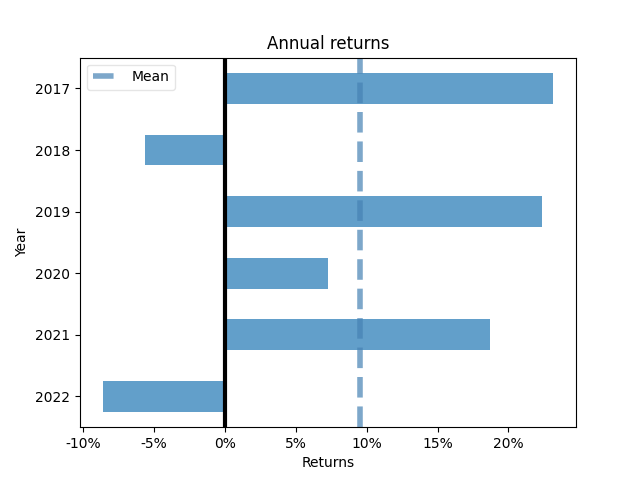
\includegraphics[width=\linewidth]{image/figure/annual_returns_dji}
            \caption{The DJI index}
        \end{subfigure}

        %
        \caption{The monthly returns.}
        \label{fig:month_annual_returns}
    \end{figure}

    \subsection{Hyperparameters}\label{subsec:hyperparameters}
    The hyperparameters include various parameters related to the learning algorithm and the environment, such as learning rate, batch size, number of steps, and the coefficients for the value function and entropy.

    \subsubsection{Hyperparameter tuning}
    Hyperparameter tuning is the process of finding the best set of hyperparameters that maximize the performance of a machine learning model. In this case, the hyperparameter sweep was performed on 27 hyperparameters using the wandb (Weights and Biases) sweep, which helps to track and visualize the training process. The hyperparameters were chosen based on their potential impact on the performance of the model and to minimize \emph{train/loss}, and the range of values for each hyperparameter was determined based on prior knowledge and experimentation.

    The sweep was performed with 5 different reinforcement learning algorithms, including A2C, PPO, SAC, DDPG, and TD3, and each algorithm was trained on 3 different datasets. The hyperparameters for each algorithm and dataset were chosen randomly from the given range or values:
    \begin{center}
        \begin{tabular}{|l|c|}
            \hline
            \textbf{Parameter}        & \textbf{Values/range}                           \\ \hline
            learning\_rate            & <0.0001, 0.01>                                  \\ \hline
            n\_steps                  & [32, 64, 128, 256, 512, 1024, 2048]             \\ \hline
            gamma                     & <0.9, 0.999>                                    \\ \hline
            gae\_lambda               & <0.8, 0.999>                                    \\ \hline
            ent\_coef                 & <0.0001, 0.01>                                  \\ \hline
            vf\_coef                  & <0.0001, 0.01>                                  \\ \hline
            max\_grad\_norm           & <0.5, 0.99>                                     \\ \hline
            rms\_prop\_eps            & <0.0001, 0.01>                                  \\ \hline
            sde\_sample\_freq         & <4, 32>                                         \\ \hline
            batch\_size               & [32, 64, 128, 256, 512, 1024, 2048, 4096, 8192] \\ \hline
            n\_epochs                 & <1, 10>                                         \\ \hline
            clip\_range               & <0.1, 0.3>                                      \\ \hline
            clip\_range\_vf           & [None, 0.05, 0.1, 0.15, 0.2]                    \\ \hline
            target\_kl                & <0.01, 0.05>                                    \\ \hline
            buffer\_size              & [1000, 2000, 3000, 4000, 5000]                  \\ \hline
            learning\_starts          & <100, 1000>                                     \\ \hline
            tau                       & <0.001, 0.01>                                   \\ \hline
            train\_freq               & <1, 4>                                          \\ \hline
            gradient\_steps           & <1, 4>                                          \\ \hline
            target\_update\_interval  & <1, 4>                                          \\ \hline
            target\_entropy           & <0.1, 0.2>                                      \\ \hline
            policy\_delay             & <1, 4>                                          \\ \hline
            target\_policy\_noise     & <0.1, 0.2>                                      \\ \hline
            target\_noise\_clip       & <0.1, 0.2>                                      \\ \hline
            exploration\_fraction     & <0.1, 0.2>                                      \\ \hline
            exploration\_initial\_eps & <0.1, 0.2>                                      \\ \hline
            exploration\_final\_eps   & <0.1, 0.2>                                      \\ \hline
        \end{tabular}
    \end{center}

    The training was repeated 10 times for each combination of 5 algorithms, 3 datasets and 10 repetitions (of random hyperparameters) for each combination. The average training and testing time was 1 hour per run, the total training time was 150 hours. The results of the hyperparameter testing are shown in the graphs where we choose several the worst models and several the best models to compare and analyze the performance of the agent, given the hyperparameters~\crefrange{fig:wb-chart1}{fig:wb-chart3}.

    \subsubsection{Best and worst hyperparameters}\label{subsubsec:best-and-worst-hyperparameters}
    The performance is being evaluated based on the \emph{test/total\_reward} attribute. The value of this attribute is being used to distinguish individual training runs, and the color of the curve represents the value of this attribute. The higher the value of \emph{test/total\_reward}, the curve is colored in \textcolor[RGB]{255,128,0}{orange} indicating better performance. On the other hand, the lower the value of \emph{test/total\_reward}, the curve is colored in \textcolor[RGB]{100,0,200}{purple} for poor performance. By examining the graphs presented in~\crefrange{fig:wb-chart1}{fig:wb-chart3}, we can identify the optimal parameters for the agent to achieve peak performance.

    \paragraph{Performance Metric}
    The initial value of \emph{test/total\_reward} is set to $1$, and its value is calculated as the cumulative product of the rewards obtained by the agent during the testing phase, as per equation~\ref{eq:portfolio-value}.

    For instance, if the agent receives rewards of $0.9$ and $1$ in the first step, then the value of \emph{test/total\_reward} would be $0.9 \times 1 = 0.9$ in the second step. If in the second step the agent receives rewards of $1.1$, then the value of \emph{test/total\_reward} would be $0.9 \times 1.1 = 0.99$ in the third step, and so on. Thus, if the final value of \emph{test/total\_reward} is $1.9$, it indicates that the agent received a total reward of $0.9$ over all the steps, which is equivalent to a portfolio return of $90\%$ over the testing period.

    \newpage
    \begin{figure}[h!]
        \centering
        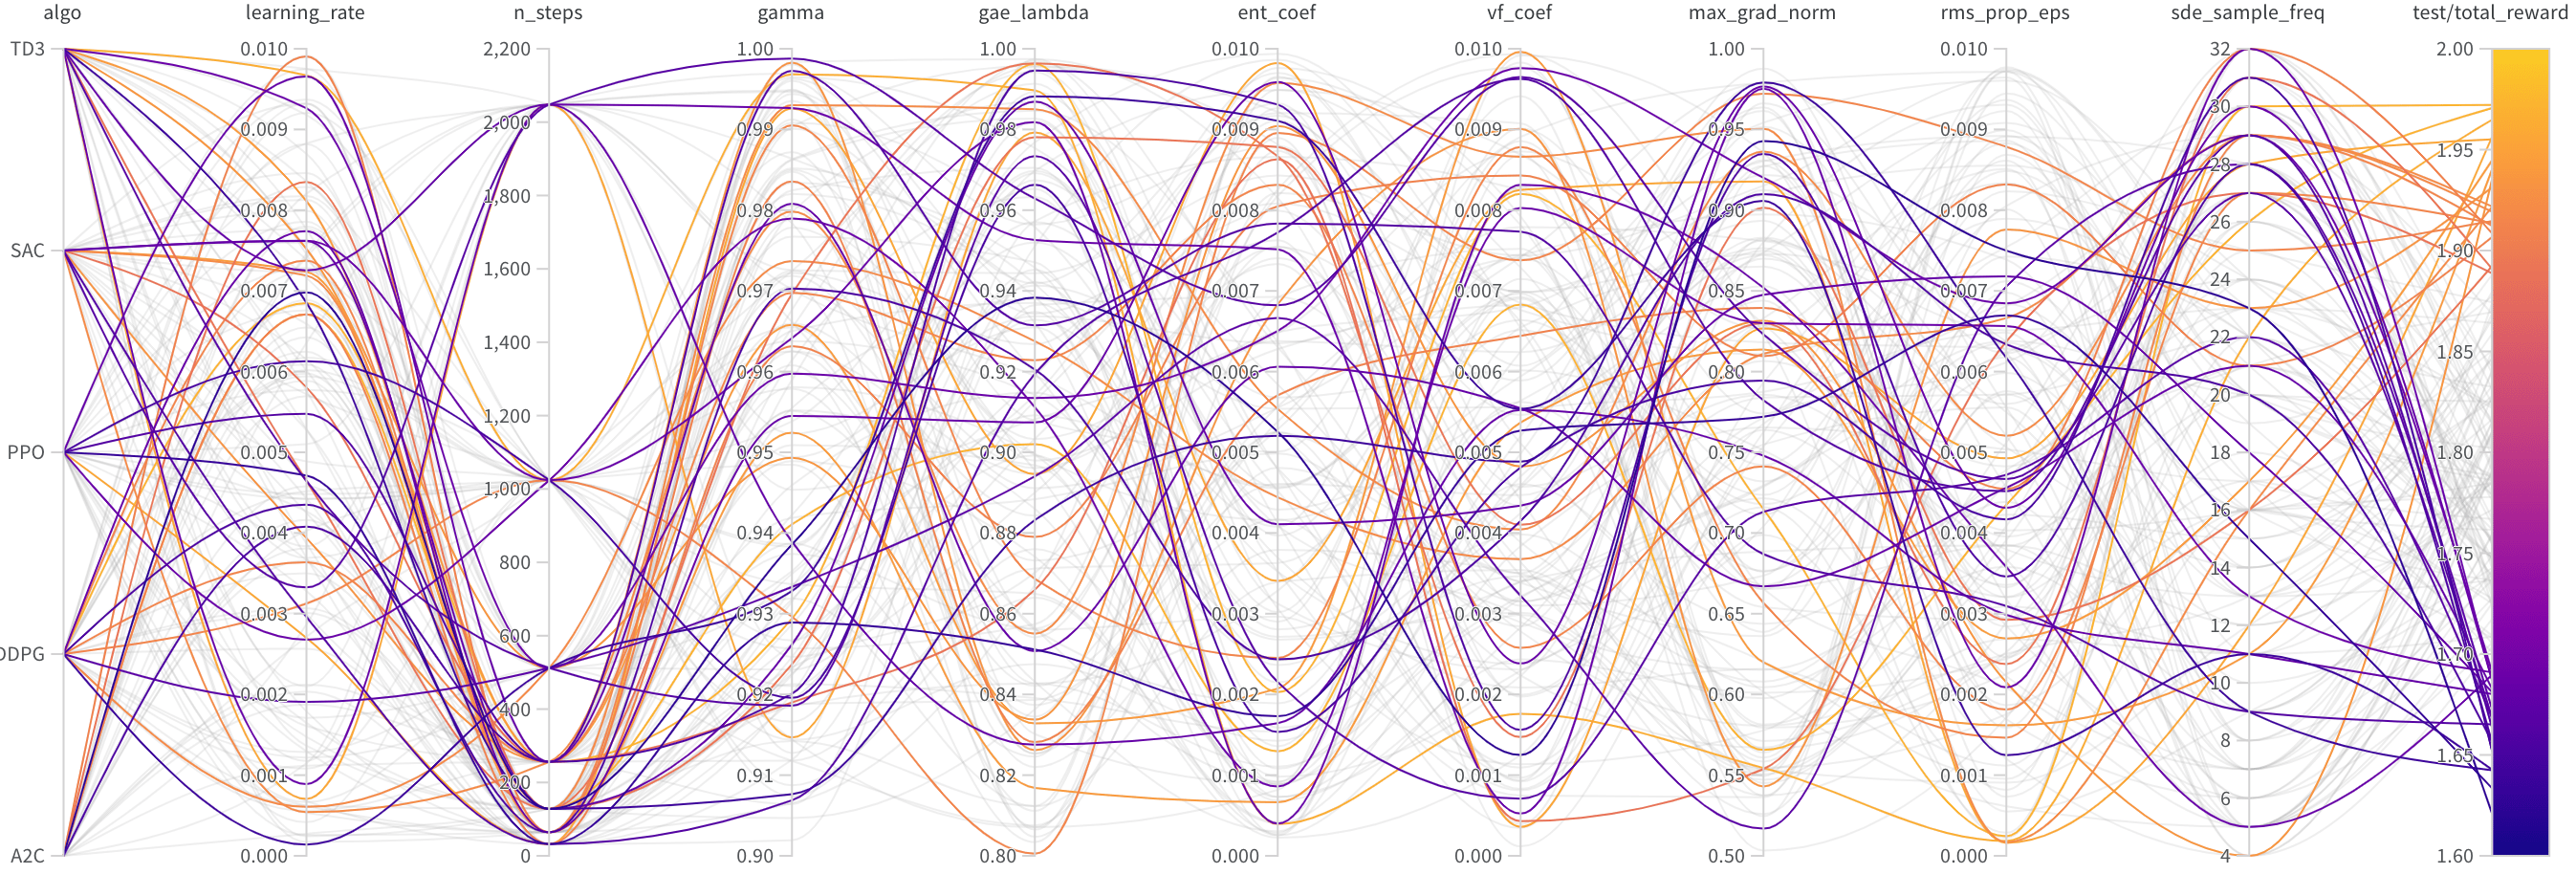
\includegraphics[width=\linewidth, height=0.2\paperheight]{image/wandb/wb1}
        \caption{W\&B Chart of parameters and their performance}
        \label{fig:wb-chart1}
    \end{figure}
    \begin{figure}[h!]
        \centering
        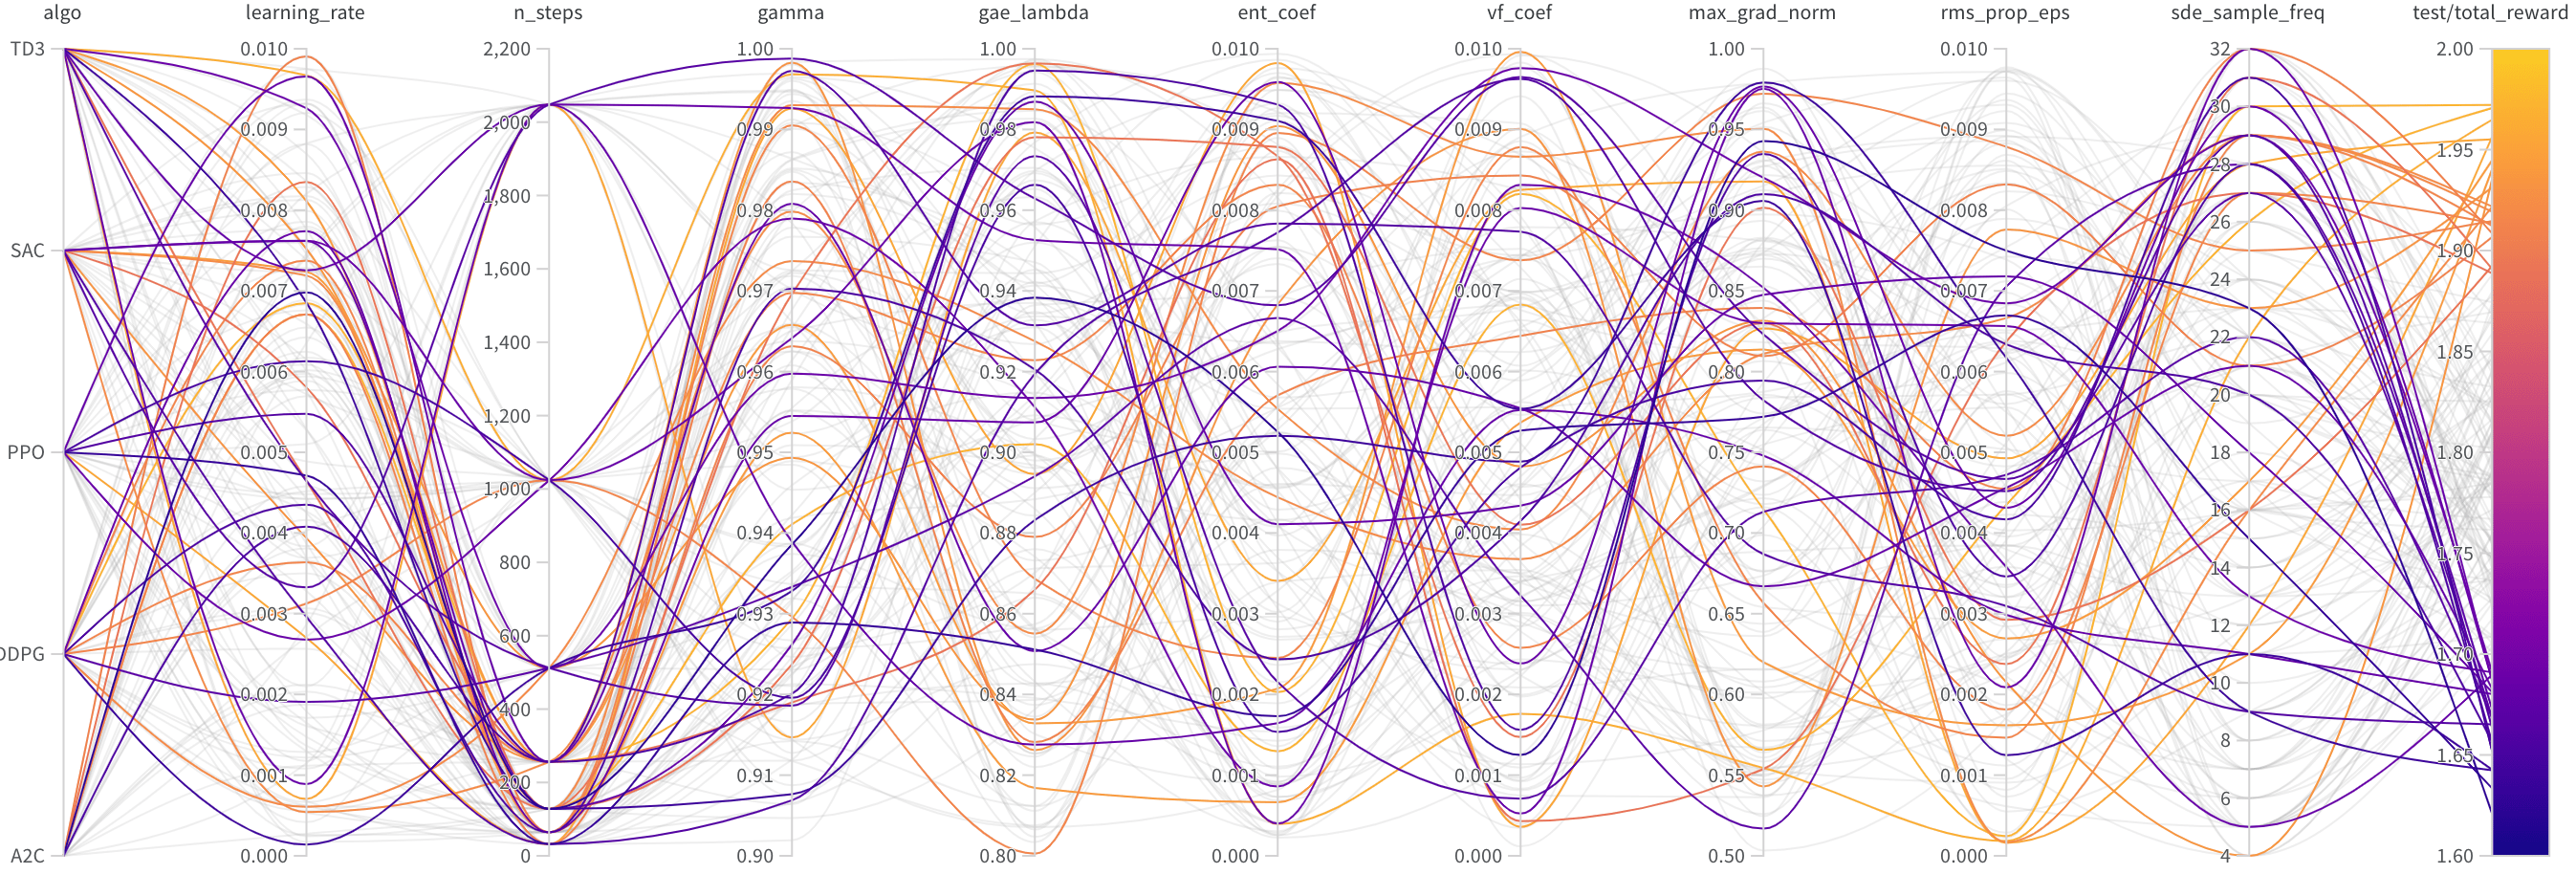
\includegraphics[width=\linewidth, height=0.2\paperheight]{image/wandb/wb1}
        \caption{W\&B Chart of parameters and their performance}
        \label{fig:wb-chart2}
    \end{figure}
    \begin{figure}[h!]
        \centering
        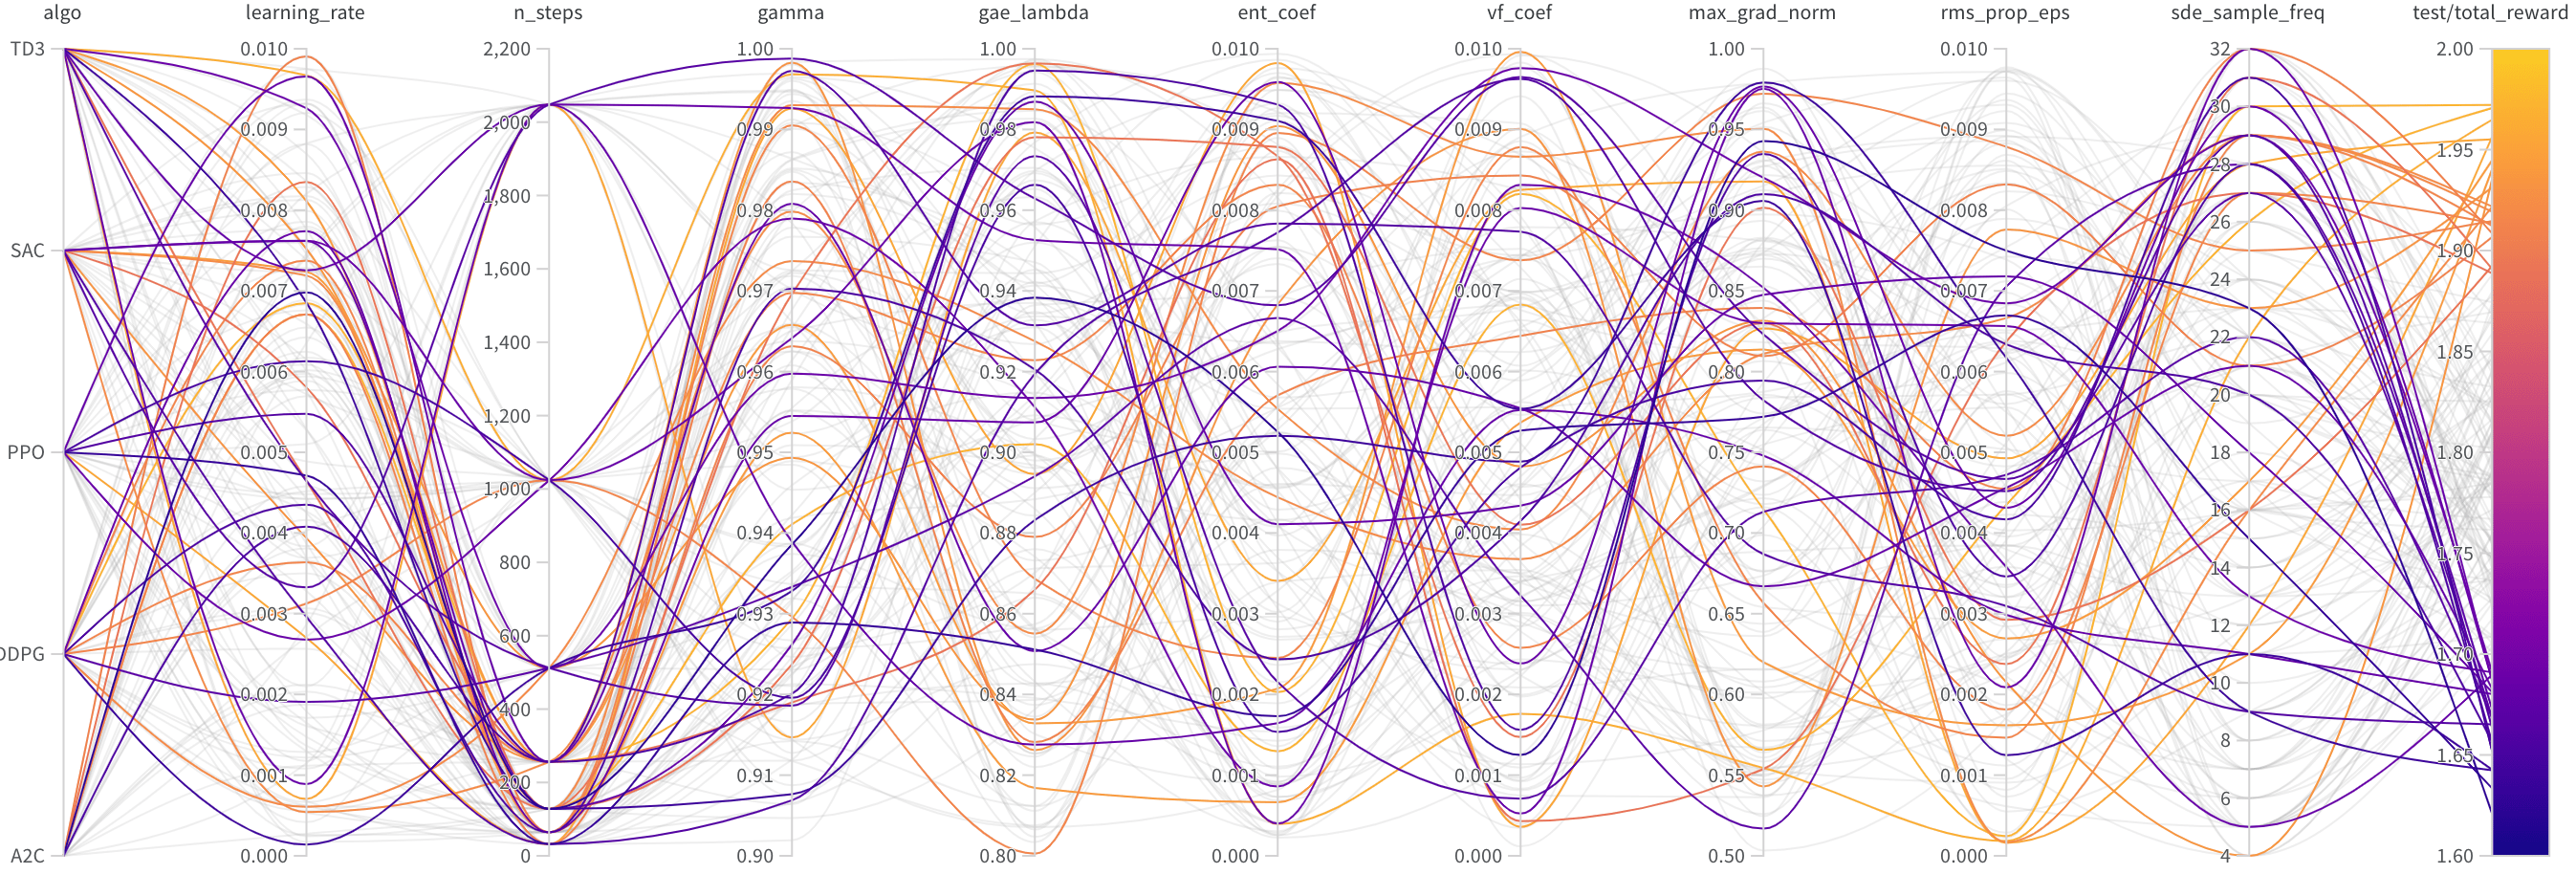
\includegraphics[width=\linewidth, height=0.2\paperheight]{image/wandb/wb1}
        \caption{W\&B Chart of parameters and their performance}
        \label{fig:wb-chart3}
    \end{figure}

    The following table shows the hyperparameters of the 2 best and 2 worst trained models:
    \begin{table}[!ht]
        \centering
        \label{tab:best-worst-hyperparameters}
        \begin{tabular}{|l||l|l||l|l|}
            \hline
            \textbf{Run ID}                    & p3irnh80                                     & 8tml2ozg                                     & zfjr0ks0                                     & pky1wslb                                     \\ \hline
            \textbf{algo}                      & DDPG                                         & A2C                                          & A2C                                          & PPO                                          \\ \hline
            \textbf{learning\_rate}            & 0.00685                                      & 0.00671                                      & 0.00698                                      & 0.00471                                      \\ \hline
            \textbf{n\_steps}                  & 256                                          & 128                                          & 128                                          & 32                                           \\ \hline
            \textbf{gamma}                     & 0.9294                                       & 0.94108                                      & 0.93858                                      & 0.9289                                       \\ \hline
            \textbf{gae\_lambda}               & 0.99624                                      & 0.90203                                      & 0.9383                                       & 0.85115                                      \\ \hline
            \textbf{ent\_coef}                 & 0.00203                                      & 0.0013                                       & 0.00525                                      & 0.00173                                      \\ \hline
            \textbf{vf\_coef}                  & 0.0082                                       & 0.00683                                      & 0.00125                                      & 0.00527                                      \\ \hline
            \textbf{max\_grad\_norm}           & 0.71475                                      & 0.56558                                      & 0.94281                                      & 0.77201                                      \\ \hline
            \textbf{rms\_prop\_eps}            & 0.00024                                      & 0.00435                                      & 0.0075                                       & 0.0067                                       \\ \hline
            \textbf{sde\_sample\_freq}         & 30                                           & 26                                           & 23                                           & 15                                           \\ \hline
            \textbf{batch\_size}               & 128                                          & 64                                           & 8192                                         & 64                                           \\ \hline
            \textbf{n\_epochs}                 & 5                                            & 8                                            & 7                                            & 8                                            \\ \hline
            \textbf{clip\_range}               & 0.18938                                      & 0.19559                                      & 0.2274                                       & 0.22578                                      \\ \hline
            \textbf{clip\_range\_vf}           & 0.05                                         & ~                                            & 0.15                                         & 0.05                                         \\ \hline
            \textbf{target\_kl}                & 0.02394                                      & 0.04957                                      & 0.03176                                      & 0.03337                                      \\ \hline
            \textbf{buffer\_size}              & 2000                                         & 5000                                         & 2000                                         & 2000                                         \\ \hline
            \textbf{learning\_starts}          & 387                                          & 163                                          & 569                                          & 165                                          \\ \hline
            \textbf{tau}                       & 0.00815                                      & 0.00461                                      & 0.00269                                      & 0.00469                                      \\ \hline
            \textbf{train\_freq}               & 2                                            & 2                                            & 3                                            & 2                                            \\ \hline
            \textbf{gradient\_steps}           & 1                                            & 3                                            & 1                                            & 3                                            \\ \hline
            \textbf{target\_update\_interval}  & 3                                            & 2                                            & 4                                            & 2                                            \\ \hline
            \textbf{target\_entropy}           & 0.19013                                      & 0.15826                                      & 0.18233                                      & 0.13979                                      \\ \hline
            \textbf{policy\_delay}             & 2                                            & 4                                            & 2                                            & 3                                            \\ \hline
            \textbf{target\_policy\_noise}     & 0.11459                                      & 0.15052                                      & 0.10674                                      & 0.12649                                      \\ \hline
            \textbf{target\_noise\_clip}       & 0.18538                                      & 0.10527                                      & 0.18672                                      & 0.14197                                      \\ \hline
            \textbf{exploration\_fraction}     & 0.12082                                      & 0.10871                                      & 0.16125                                      & 0.16269                                      \\ \hline
            \textbf{exploration\_final\_eps}   & 0.18574                                      & 0.10366                                      & 0.10618                                      & 0.19131                                      \\ \hline
            \textbf{exploration\_initial\_eps} & 0.16609                                      & 0.10003                                      & 0.16434                                      & 0.1039                                       \\ \hline
            \textbf{test/total\_reward}        & \textcolor[RGB]{50,150,50}{\textbf{1.97214}} & \textcolor[RGB]{50,150,50}{\textbf{1.97061}} & \textcolor[RGB]{150,50,50}{\textbf{1.62093}} & \textcolor[RGB]{150,50,50}{\textbf{1.63348}} \\ \hline
        \end{tabular}
        \caption{Best and worst model and their training hyperparameters. All hyperparameters are also available online URL: \url{https://wandb.ai/investai/portfolio-allocation} with much more details and experiments.}
    \end{table}

    \subsection{Datasets}\label{subsec:datasets}
    In the previous chapter we compare models based on the \emph{test/total\_reward} of the agent, comparing training hyperparameters Now we look and compare model performance based on the dataset used. We compare the same models (2 best and 2 worst models) used in the previous section in~\cref{tab:best-worst-datasets}, and we also include the best and worst model from the \emph{Fundamental Analysis} dataset and \emph{Technical Analysis} in~\cref{subsec:datasets}. The results are shown in Table~\cref{tab:best-worst-datasets}.
    \begin{table}[!ht]
        \centering
        \label{tab:best-worst-datasets}
        \begin{tabular}{|l|l|l|}
            \hline
            \textbf{Run ID} & \textbf{Dataset Name} & \textbf{test/total\_reward}                \\ \hline
            p3irnh80        & Combined              & \textcolor[RGB]{50,150,50}{\textbf{1.972}} \\ \hline
            8tml2ozg        & Combined              & \textcolor[RGB]{50,150,50}{\textbf{1.970}} \\ \hline
            zfjr0ks0        & Fundamental Analysis  & \textcolor[RGB]{150,50,50}{\textbf{1.620}} \\ \hline
            pky1wslb        & Combined              & \textcolor[RGB]{150,50,50}{\textbf{1.633}} \\ \hline
        \end{tabular}
        \caption{Permormance of the datasets used for training the two best and two worst models used in the previous section for comparing hyperparameters as well.}
    \end{table}

    \begin{table}[!ht]
        \centering
        \label{tab:worst-datasets}
        \begin{tabular}{|l|l|l|}
            \hline
            \textbf{Run ID} & \textbf{Dataset Name} & \textbf{test/total\_reward}                \\ \hline
            zfjr0ks0        & Fundamental Analysis  & \textcolor[RGB]{150,50,50}{\textbf{1.620}} \\ \hline
            pky1wslb        & Combined              & \textcolor[RGB]{150,50,50}{\textbf{1.633}} \\ \hline
            2161deh4        & Technical Analysis    & \textcolor[RGB]{150,50,50}{\textbf{1.642}} \\ \hline
            ipl1v8io        & Technical Analysis    & \textcolor[RGB]{150,50,50}{\textbf{1.643}} \\ \hline
            2161deh4        & Technical Analysis    & \textcolor[RGB]{150,50,50}{\textbf{1.642}} \\ \hline
            2161deh4        & Technical Analysis    & \textcolor[RGB]{150,50,50}{\textbf{1.642}} \\ \hline
        \end{tabular}
        \caption{The datasets with the poorest performing models.}
    \end{table}

    \begin{table}[!ht]
        \centering
        \label{tab:best-datasets}
        \begin{tabular}{|l|l|l|}
            \hline
            \textbf{Run ID} & \textbf{Dataset Name} & \textbf{test/total\_reward}                \\ \hline
            p3irnh80        & Combined              & \textcolor[RGB]{50,150,50}{\textbf{1.972}} \\ \hline
            8tml2ozg        & Combined              & \textcolor[RGB]{50,150,50}{\textbf{1.970}} \\ \hline
            geaioz9h        & Fundamental Analysis  & \textcolor[RGB]{50,150,50}{\textbf{1.965}} \\ \hline
            8iq9e37s        & Combined              & \textcolor[RGB]{50,150,50}{\textbf{1.956}} \\ \hline
            y3zz2sv3        & Combined              & \textcolor[RGB]{50,150,50}{\textbf{1.955}} \\ \hline
            4qr3nk43        & Fundamental Analysis  & \textcolor[RGB]{50,150,50}{\textbf{1.945}} \\ \hline
        \end{tabular}
        \caption{The datasets with the best performing models.}
    \end{table}

    Based on the~\crefrange{tab:best-worst-datasets}{tab:best-datasets} it appears that the performance of the models is highly dependent on the choice of hyperparameters, making it difficult to determine the worst dataset. However, it seems clear that when the hyperparameters are well-tuned, the \emph{Combined Dataset} performs the best, while the \emph{Fundamental Dataset} also performs well.

    All the information, including hyperparameters, datasets, and other details, are available online at the following URL: \url{https://wandb.ai/investai/portfolio-allocation}. The website contains extensive information about the experiments and includes many more details.

    \subsection{Robustness Testings}

    \newpage

    \subsubsection{Overall Performance and Statistics}
%    TODO: Table performance with stats from pyfolio
    In the~\cref{tab:stats} we can see overall performance and statistics of the models. The \textbf{bold} values are the best results for each metric. As we can se our model outperform almost all other models/strategies in almost all metrics.

    TODO describe this table in details

    \subsection{Against the Indexes, Strategies}

%    \begin{landscape}
    \begin{table}[ht!]
        \centering
        \caption{Performance metrics of the models, indexes and strategies}
        \label{tab:stats}
        {\footnotesize
            \begin{tabular}{*{10}{|m{0.075\linewidth}|}}
                \toprule
                & \bfseries The lowest Total Reward & \bfseries The highest Total Reward   & \bfseries \^DJI & \bfseries \^GSPC & \bfseries \^IXIC & \bfseries \^RUT & \bfseries Max Sharpe ratio & \bfseries Min Variance \\[0.5cm]
                \midrule
                \bfseries Annual return       & 0.085                             & \color[HTML]{00F000} \bfseries 0.122 & 0.089                                 & 0.094            & 0.116 & 0.043 & 0.093 & 0.092 \\[0.5cm]
                \bfseries Cum. returns        & 0.621                             & \color[HTML]{00F000} \bfseries 0.972 & 0.654                                 & 0.695            & 0.911 & 0.284 & 0.686 & 0.683 \\[0.5cm]
                \bfseries Annual volatility   & 0.181                             & 0.188                                & 0.202                                 & 0.203            & 0.239            & \color[HTML]{00F000} \bfseries 0.253 & 0.158 & 0.158 \\[0.5cm]
                \bfseries Sharpe ratio        & 0.543                             & \color[HTML]{00F000} \bfseries 0.706 & 0.525                                 & 0.544            & 0.581 & 0.295 & 0.641 & 0.640 \\[0.5cm]
                \bfseries Calmar ratio        & 0.288                             & \color[HTML]{00F000} \bfseries 0.391 & 0.241                                 & 0.276            & 0.325 & 0.101 & 0.350 & 0.349 \\[0.5cm]
                \bfseries Stability           & 0.855                             & \color[HTML]{00F000} \bfseries 0.913 & 0.798                                 & 0.845            & 0.820 & 0.461 & 0.905 & 0.905 \\[0.5cm]
                \bfseries Max drawdown        & -0.297                            & -0.312                               & -0.371                                & -0.339           & -0.357           & -0.431                               & \color[HTML]{00F000} \bfseries -0.265 & \color[HTML]{00F000} \bfseries -0.265 \\[0.5cm]
                \bfseries Omega ratio         & 1.118                             & \color[HTML]{00F000} \bfseries 1.158 & 1.114                                 & 1.115            & 1.115 & 1.057 & 1.136 & 1.135 \\[0.5cm]
                \bfseries Sortino ratio       & 0.763                             & \color[HTML]{00F000} \bfseries 0.994 & 0.723                                 & 0.751            & 0.802 & 0.404 & 0.907 & 0.904 \\[0.5cm]
                \bfseries Skew                & -0.249                            & -0.312                               & -0.593                                & -0.549           & -0.465           & -0.782                               & -0.246                                & \color[HTML]{00F000} \bfseries -0.240 \\[0.5cm]
                \bfseries Kurtosis            & 16.819                            & 19.569                               & \color[HTML]{00F000} \bfseries 19.640 & 14.205           & 7.418 & 10.450 & 14.315 & 14.286 \\[0.5cm]
                \bfseries Tail ratio          & 0.883                             & 0.883                                & 0.891                                 & 0.859            & 0.862            & \color[HTML]{00F000} \bfseries 0.984 & 0.937 & 0.930 \\[0.5cm]
                \bfseries Daily value at risk & -0.022                            & -0.023                               & -0.025                                & -0.025           & -0.030           & -0.032                               & \color[HTML]{00F000} \bfseries -0.019 & \color[HTML]{00F000} \bfseries -0.019 \\[0.5cm]
                \bfseries Beta                & 0.879                             & 0.921                                & 1.000                                 & 0.966            & 1.007            & \color[HTML]{00F000} \bfseries 1.083 & 0.636 & 0.636 \\[0.5cm]
                \bfseries Alpha               & 0.005                             & \color[HTML]{00F000} \bfseries 0.036 & 0.000                                 & 0.008            & 0.032            & -0.039 & 0.034 & 0.034 \\[0.5cm]
                \bottomrule
            \end{tabular}
        }
    \end{table}
    %    \end{landscape}

    \subsection{Against the Other Publicly Available RL Agents}\label{subsec:against-the-other-publicly-available-rl-agents}


    \newpage


    \section{Summary}\label{sec:summary}
    In this chapter, we conducted empirical experiments to evaluate how well a Deep Reinforcement Learning (DRL) agent can perform in the portfolio management task. Our results show that DRL has a huge potential in portfolio allocation as it can outperform common strategies and indexes. We used DRL algorithms to explore the relationship between the reward (i.e., portfolio return) and the input (i.e., features) and measured the prediction power using portfolio metrics. We found that the Fundamental Features or a combination of Fundamental and Technical Analysis features can effectively describe the environment and be used to train DRL agents.

    Portfolio management is a challenging task that requires a lot of data, which is often expensive and difficult to obtain. Our Stock Portfolio Allocation Environment, modeled using MDP, aims to identify how stocks are valued and which State Space features affect price movements. We assume that the Financial Market operates like any other market where the price of a stock or asset increases when people buy it and decreases when people sell it. Therefore, our model attempts to predict how much each feature affects future price movements (people's interest to buy/sell). Since the Stock Market is predominantly controlled by "Big Money" players such as banks and hedge funds, we believe that our research is crucial for portfolio managers to improve their decision-making capabilities.

    In addition to the future work mentioned earlier, we see a great opportunity to extend our model by incorporating a system that automatically places orders to the broker based on the weight predicted by our model. This would streamline the entire process of portfolio management and eliminate the need for manual intervention.

    Furthermore, we believe that our model can benefit from the inclusion of additional features such as sentiment analysis, macroeconomic factors, and industry-specific factors. The inclusion of these features can help our model to better capture the market's behavior and improve its performance.

    Another area of improvement that we believe warrants further exploration is the reward function. While our experiments have shown that the reward function we used was effective to some extent, we acknowledge that it may not capture all the nuances of the market. Therefore, we recommend exploring alternative reward functions that can better account for the goodness or badness of actions taken by the agent.

    Overall, we believe that our study has demonstrated the potential of DRL in portfolio allocation, but there are still many avenues for improvement and further research. By incorporating these future works, we can enhance the performance of our model and make it more suitable for real-world applications.


    % TODO: Dividends are not considered

\end{document}
